% Options for packages loaded elsewhere
\PassOptionsToPackage{unicode}{hyperref}
\PassOptionsToPackage{hyphens}{url}
%
\documentclass[
]{article}
\usepackage{lmodern}
\usepackage{amssymb,amsmath}
\usepackage{ifxetex,ifluatex}
\ifnum 0\ifxetex 1\fi\ifluatex 1\fi=0 % if pdftex
  \usepackage[T1]{fontenc}
  \usepackage[utf8]{inputenc}
  \usepackage{textcomp} % provide euro and other symbols
\else % if luatex or xetex
  \usepackage{unicode-math}
  \defaultfontfeatures{Scale=MatchLowercase}
  \defaultfontfeatures[\rmfamily]{Ligatures=TeX,Scale=1}
\fi
% Use upquote if available, for straight quotes in verbatim environments
\IfFileExists{upquote.sty}{\usepackage{upquote}}{}
\IfFileExists{microtype.sty}{% use microtype if available
  \usepackage[]{microtype}
  \UseMicrotypeSet[protrusion]{basicmath} % disable protrusion for tt fonts
}{}
\makeatletter
\@ifundefined{KOMAClassName}{% if non-KOMA class
  \IfFileExists{parskip.sty}{%
    \usepackage{parskip}
  }{% else
    \setlength{\parindent}{0pt}
    \setlength{\parskip}{6pt plus 2pt minus 1pt}}
}{% if KOMA class
  \KOMAoptions{parskip=half}}
\makeatother
\usepackage{xcolor}
\IfFileExists{xurl.sty}{\usepackage{xurl}}{} % add URL line breaks if available
\IfFileExists{bookmark.sty}{\usepackage{bookmark}}{\usepackage{hyperref}}
\hypersetup{
  hidelinks,
  pdfcreator={LaTeX via pandoc}}
\urlstyle{same} % disable monospaced font for URLs
\usepackage[margin=1in]{geometry}
\usepackage{graphicx}
\makeatletter
\def\maxwidth{\ifdim\Gin@nat@width>\linewidth\linewidth\else\Gin@nat@width\fi}
\def\maxheight{\ifdim\Gin@nat@height>\textheight\textheight\else\Gin@nat@height\fi}
\makeatother
% Scale images if necessary, so that they will not overflow the page
% margins by default, and it is still possible to overwrite the defaults
% using explicit options in \includegraphics[width, height, ...]{}
\setkeys{Gin}{width=\maxwidth,height=\maxheight,keepaspectratio}
% Set default figure placement to htbp
\makeatletter
\def\fps@figure{htbp}
\makeatother
\setlength{\emergencystretch}{3em} % prevent overfull lines
\providecommand{\tightlist}{%
  \setlength{\itemsep}{0pt}\setlength{\parskip}{0pt}}
\setcounter{secnumdepth}{-\maxdimen} % remove section numbering
\usepackage{ctex}
\usepackage{xcolor}
\usepackage{fancyhdr}
\pagestyle{plain}
\usepackage{sectsty}
\definecolor{glaucous}{rgb}{0.38, 0.51, 0.71}
\definecolor{lavenderblush}{rgb}{1.0, 0.94, 0.96}
\usepackage{enumitem}% http://ctan.org/pkg/enumitem
\usepackage[empty]{fullpage}% http://ctan.org/pkg/fullpage
\usepackage{color}% http://ctan.org/pkg/color
\usepackage{hyperref}% http://ctan.org/pkg/hyperref
\usepackage{geometry}
\geometry{a4paper,left=0.5cm,right=0.5cm,top=0.3cm,bottom=0.3cm}
\usepackage{blindtext}
\usepackage[center]{caption}
\usepackage[font=Large]{caption}
\usepackage{subfigure}
\usepackage{float}
\usepackage{graphicx}
\usepackage{booktabs}
\usepackage[justification=centering]{caption}
\usepackage{threeparttable}
\usepackage{longtable}
\usepackage{array}
\usepackage{multirow}
\usepackage{wrapfig}
\usepackage{float}
\usepackage{colortbl}
\usepackage{pdflscape}
\usepackage{tabu}
\usepackage{threeparttable}
\usepackage{threeparttablex}
\usepackage[normalem]{ulem}
\usepackage{makecell}
\usepackage{xcolor}
\linespread{1.15}
\setlength{\parskip}{1em}
\setlength{\footskip}{20pt}
\usepackage{booktabs}
\usepackage{longtable}
\usepackage{array}
\usepackage{multirow}
\usepackage{wrapfig}
\usepackage{float}
\usepackage{colortbl}
\usepackage{pdflscape}
\usepackage{tabu}
\usepackage{threeparttable}
\usepackage{threeparttablex}
\usepackage[normalem]{ulem}
\usepackage{makecell}
\usepackage{xcolor}

\author{}
\date{\vspace{-2.5em}}

\begin{document}

\captionsetup[figure]{name={图},labelsep=space} 
\captionsetup[table]{name={表},labelsep=space} 
\fontsize{22}{22}
\selectfont
\vspace{-10truemm}

\newcommand{\resheading}[1]{%
  \noindent\fcolorbox{lavenderblush}{lavenderblush}{\makebox[\dimexpr\textwidth-2\fboxsep-2\fboxrule][l]{\textbf{~#1}}}%
}

\begin{center}

\includegraphics[height=2cm]{./input/logo2.png} 
\end{center}

\begin{center}
\fontsize{45}{45}
\textcolor{glaucous}{\textbf{新冠早报}}
\end{center}

\begin{center}
\fontsize{22}{22}
{\textcolor{glaucous}{\textbf{第13期 \space 4月8日}}}
\end{center}

%
  \noindent\fcolorbox{lavenderblush}{lavenderblush}{\makebox[\dimexpr\textwidth-2\fboxsep-2\fboxrule][l]{\textbf{~\Huge 每日新闻}}}%

\hypertarget{section}{%
\subsection{\texorpdfstring{\textcolor{glaucous}{\Huge 国际}}{}}\label{section}}

\textbf{\textcolor{glaucous}{英国广播公司(BBC)}}:
\textbf{G20允许最贫穷国家延期偿付高达120亿美元债务 }

当地时间4月15日,二十国集团(G20)主要经济体国家同意允许一些世界上最贫穷国家延期支付共计高达120亿美金的债务,宽限至2022年至2024年间偿还。该协议涵盖了到2020年底应支付给G20政府的款项,目的是帮助各国应对冠状病毒大流行的健康和经济影响。共有77个国家将从该协议中受益。

\textbf{\textcolor{glaucous}{盖茨基金会(Bill and Melinda Gates Foundation)}}
: \textbf{盖茨基金会再度提高赠款总额,呼吁全球合作保护民众免受疫情侵害}

当地时间4月15日,比尔及梅琳达·盖茨基金会宣布再次追加捐赠金额,以支持全球对新冠肺炎(COVID-19)疫情的响应行动。此次盖茨基金会额外赠款1.5亿美元,并承诺将动用基金会``战略投资基金''的资源,用于加快关键医疗物资的采购,帮助生命科学公司获得生产新冠肺炎相关产品所需的资金。在宣布追加赠款的同时,盖茨基金会还呼吁各国领导人携手应对疫情,确保人人享有获得诊断、治疗和疫苗的公平权利。

\textbf{\textcolor{glaucous}{福布斯新闻(Forbes)}} :
\textbf{美国部分州可能在5月1日前重启经济}

当地时间4月15日,美国疾控中心主任罗伯特·雷德菲尔德在接受采访时说,联邦政府正在筹划在5月1日之前对大约20个受新冠病毒影响较小的州放宽限制。重新开放的社区必须满足的条件包括:拥有有效的病例追踪系统、具有充足的资源以备治疗新增病例的能力、以及足够低的感染发生率。然而也有报告表示,一些社区可能需要将隔离措施进行到2022年。因此,各社区需做好间歇性采取更严格的措施的准备,以避免病毒感染``大反弹''。

\textbf{\textcolor{glaucous}{纽约时报(New York Times)}} :
\textbf{纽约州州长要求所有人在公共场所必须戴口罩 }

当地时间4月15日,纽约州州长科莫在新冠疫情新闻发布会上表示,为防止疫情扩散,他将签署一项行政命令,要求纽约州所有人在难以保持社交距离(人和人之间保持至少6英尺)的公共场合,例如乘坐公共交通时,必须用口罩或其他遮挡物覆盖面部。该行政命令在本周六生效,纽约州居民有三天的时间准备好有关物资。

\textbf{\textcolor{glaucous}{英国广播公司(BBC)}} :
\textbf{德国缓慢放宽封锁措施 }

当地时间4月15日,德国总理默克尔宣布计划将逐步放宽应对冠状病毒大流行的限制措施。默克尔表示,社交距离规则将保留到至少5月3日,在商店和公共交通工具上也建议坚持使用口罩。但从下周开始,部分商店可以开门营业,从5月4日起,学校也将逐渐开始重新开放。

\textbf{\textcolor{glaucous}{英国广播公司(BBC)}} :
\textbf{韩国举行国会选举 选民戴口罩及塑胶手套投票 }

当地时间4月15日,韩国举行国会选举。选民在投票时需要严守防疫规定,包括戴口罩及塑胶手套,以及彼此之间保持1公尺以上的距离。经过消毒的14000个投票点于上午6点开放,选民抵达后还要需要接受体温检测,37.5度以上的选民将被安排到特别设置的小隔间投票。新冠疫情爆发以来,许多国家相继推迟选举时程,韩国是如期举行选举的首批国家之一。

\hypertarget{section-1}{%
\subsection{\texorpdfstring{\textcolor{glaucous}{\Huge 国内}}{}}\label{section-1}}

\textbf{\textcolor{glaucous}{央视新闻}}:
\textbf{影剧院、游戏厅等娱乐场所暂不开业 大型展览展会暂不开展 }

北京时间4月15日下午,国务院联防联控机制召开新闻发布会,中国疾控中心环境所所长施小明介绍,影剧院或者是游戏厅等娱乐性或休闲性场所暂不开业,大型的体育活动或展览展会也暂不开展。

\textbf{\textcolor{glaucous}{央视新闻}}:
\textbf{民航已安排临时航班(包机)赴疫情严重国家接回2744名中国公民}

北京时间4月15日,记者从中国民用航空局了解到,3月4日至4月12日,民航局共安排16架次临时航班协助在伊朗、意大利、英国、美国、西班牙的2744名中国公民回国,其中留学生1449名。

\hfill\break

%
  \noindent\fcolorbox{lavenderblush}{lavenderblush}{\makebox[\dimexpr\textwidth-2\fboxsep-2\fboxrule][l]{\textbf{~\Huge 疫情观察}}}%

\begin{Large}
{数据源:约翰霍普金斯大学,The COVID Tracking Project \\ 数据截止至:北京时间3月28日 早4:00}
\end{Large}

\hypertarget{section-2}{%
\section{\texorpdfstring{\textcolor{glaucous}{\Huge 一、世界疫情}}{}}\label{section-2}}

\(\quad\)截至北京时间4月16日早7:00,全球累计确诊病例已经达到2,056,055例,累计死亡134,178
例。在180多个出现确诊病例的国家或地区中,已有23个国家累计确诊超万人。除欧洲和美国以外,拉美和亚州的发展中国家的病例快速增长:印度和秘鲁确诊人数已经超过万人。非洲国家累计确诊病例已逾一万六千例。英国确诊病例已经超过中国,成为世界第六位
(表1)。

\begin{figure}[H]
\caption{世界疫情分布图} %最终文档中希望显示的图片标题
\centering
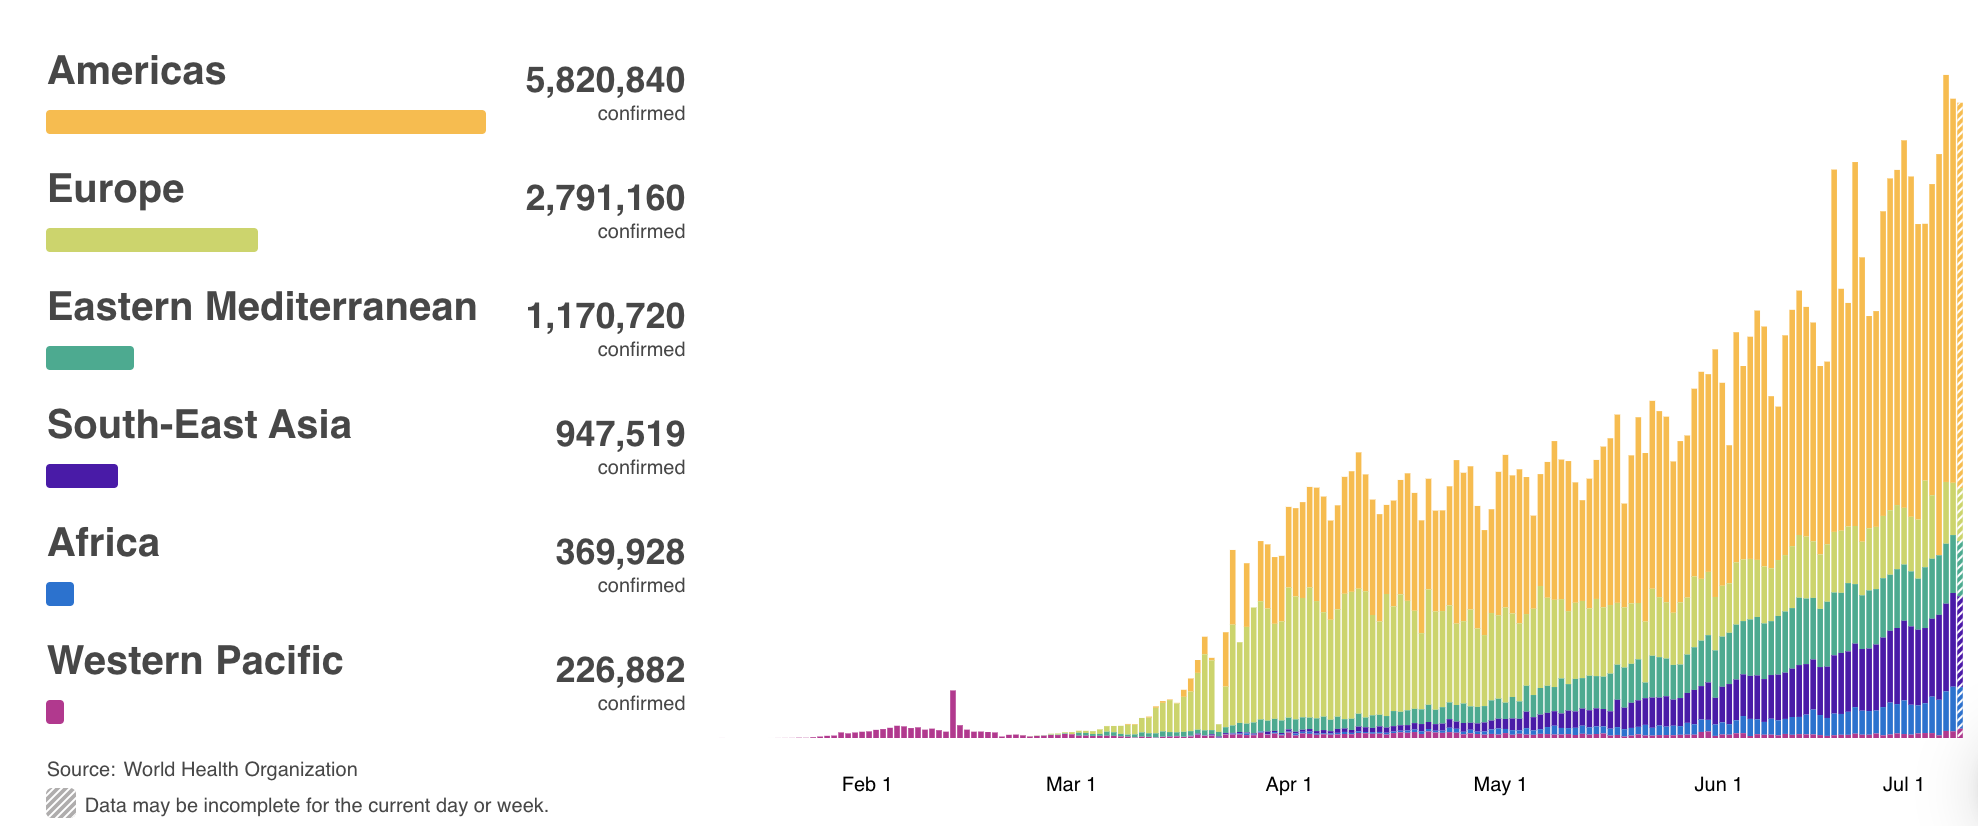
\includegraphics[]{./input/covid1.png} %插入图片,[]中设置图片大小,{}中是图片文件名
\label{} %用于文内引用的标签
\end{figure}

\begin{table}[H]
    \caption{累计确诊前十位国家}
      \vspace{-0.5\baselineskip}
      \centering \begin{table}[H]
\centering\begingroup\fontsize{18}{20}\selectfont

\begin{tabular}{rlrrr}
\toprule
  & 国家(地区) & 累计确诊病例 & 总人口 & 粗发病率\\
\midrule
\rowcolor{gray!6}  1 & 美国 US & 636,350 & 331,002,651 & 192\\
2 & 西班牙 Spain & 177,644 & 46,754,778 & 380\\
\rowcolor{gray!6}  3 & 意大利 Italy & 165,155 & 60,461,826 & 273\\
4 & 法国 France & 137,875 & 65,273,511 & 211\\
\rowcolor{gray!6}  5 & 德国 Germany & 134,753 & 83,783,942 & 161\\
6 & 英国 UK & 99,483 & 67,886,011 & 147\\
\rowcolor{gray!6}  7 & 中国 China & 83,356 & 1,439,323,776 & 6\\
 & 湖北 Hubei & 67,803 & 59,172,000 & 115\\
\rowcolor{gray!6}  8 & 伊朗 Iran & 76,389 & 83,992,949 & 91\\
9 & 土耳其 Turkey & 69,392 & 84,339,067 & 82\\
\rowcolor{gray!6}  10 & 比利时 Belgium & 33,573 & 11,589,623 & 290\\
\bottomrule
\end{tabular}
\endgroup{}
\end{table} \begin{tablenotes}
        \fontsize{15}{15}
        \selectfont
        \item 注:粗发病率定义:在一定时间内,特定范围人群中某病新发生的病例出现的频率。计算方式:(累计确诊病例/人口)×10万  %此处加入注释信息
      \end{tablenotes}
    \end{table}

\(\quad\)美国新增病例数仍居全球首位,已连续十六天日新增病例数超过两万五千人。意大利日新增病例数已经连续三日下降,西班牙和德国的日新增病例较昨日翻倍。值得注意的是,俄罗斯、巴西和比利时的病例较前日增长很快,这三个国家的累计确诊人数已突破两万例。提示欧洲、北美和南美疫情发展迅速
(表2和图2)。

\(\quad\)美国的日新增死亡病例已经接近2,500(2,494例),从4月4日至今一直为前十位国家中首位,病死率已经上升到4.5\%,疫情发展不容乐观。法国的日新增死亡病例数波动较大。今日较昨日翻倍,成为日新增死亡病例数仅次于美国的国家(1,440)例。法国病死率持续上升(12.5\%),提示该国医疗系统正面临巨大压力。意大利和西班牙的日新增死亡病例数呈波动下降趋势。英国新增死亡病例数波动上升,还有待进一步观察
(表3和图3)。

\begin{table}[H]

    \begin{minipage}{.4\linewidth}
    \centering
    \captionsetup{justification=centering}
    \caption{日新增病例前十位国家}
    \vspace{-0.5\baselineskip}
      \centering
    \captionsetup{justification=centering} \begin{table}[H]
\centering\begingroup\fontsize{12}{14}\selectfont

\begin{tabular}{rlr}
\toprule
  & 国家 & 当日新增病例\\
\midrule
\rowcolor{gray!6}  1 & 美国 US & 28,680\\
2 & 西班牙 Spain & 5,103\\
\rowcolor{gray!6}  3 & 英国 UK & 4,638\\
4 & 土耳其 Turkey & 4,281\\
\rowcolor{gray!6}  5 & 德国 Germany & 3,394\\
6 & 俄罗斯 Russia & 3,388\\
\rowcolor{gray!6}  7 & 巴西 Brazil & 3,058\\
8 & 意大利 Italy & 2,667\\
\rowcolor{gray!6}  9 & 比利时 Belgium & 2,454\\
10 & 伊朗 Iran & 1,512\\
\bottomrule
\end{tabular}
\endgroup{}
\end{table} \end{minipage}
    \begin{minipage}{.6\linewidth}
    \centering
    \captionsetup{justification=centering}
     \caption{累计死亡病例前十位国家}
     \vspace{-0.5\baselineskip}
      \centering
    \captionsetup{justification=centering} \begin{table}[H]
\centering\begingroup\fontsize{12}{14}\selectfont

\begin{tabular}{rlrrr}
\toprule
  & 国家 & 累计死亡病例 & 较昨日新增 & 病死率\%\\
\midrule
\rowcolor{gray!6}  1 & 美国 US & 28,326 & 2,494 & 4.5\\
2 & 意大利 Italy & 21,645 & 578 & 13.1\\
\rowcolor{gray!6}  3 & 西班牙 Spain & 18,708 & 652 & 10.5\\
4 & 法国 France & 17,188 & 1,440 & 12.5\\
\rowcolor{gray!6}  5 & 英国 UK & 12,894 & 765 & 13.0\\
6 & 伊朗 Iran & 4,777 & 94 & 6.3\\
\rowcolor{gray!6}  7 & 比利时 Belgium & 4,440 & 283 & 13.2\\
8 & 德国 Germany & 3,804 & 510 & 2.8\\
\rowcolor{gray!6}  9 & 中国 China & 3,346 & 1 & 4.0\\
10 & 荷兰 Netherlands & 3,145 & 190 & 11.1\\
\bottomrule
\end{tabular}
\endgroup{}
\end{table} \end{minipage} 
\end{table}

\begin{figure}[H]
\centering
\begin{minipage}[b]{0.48\linewidth}
\caption{日新增确诊病例国家趋势图\\(中国及其他前五位国家)}
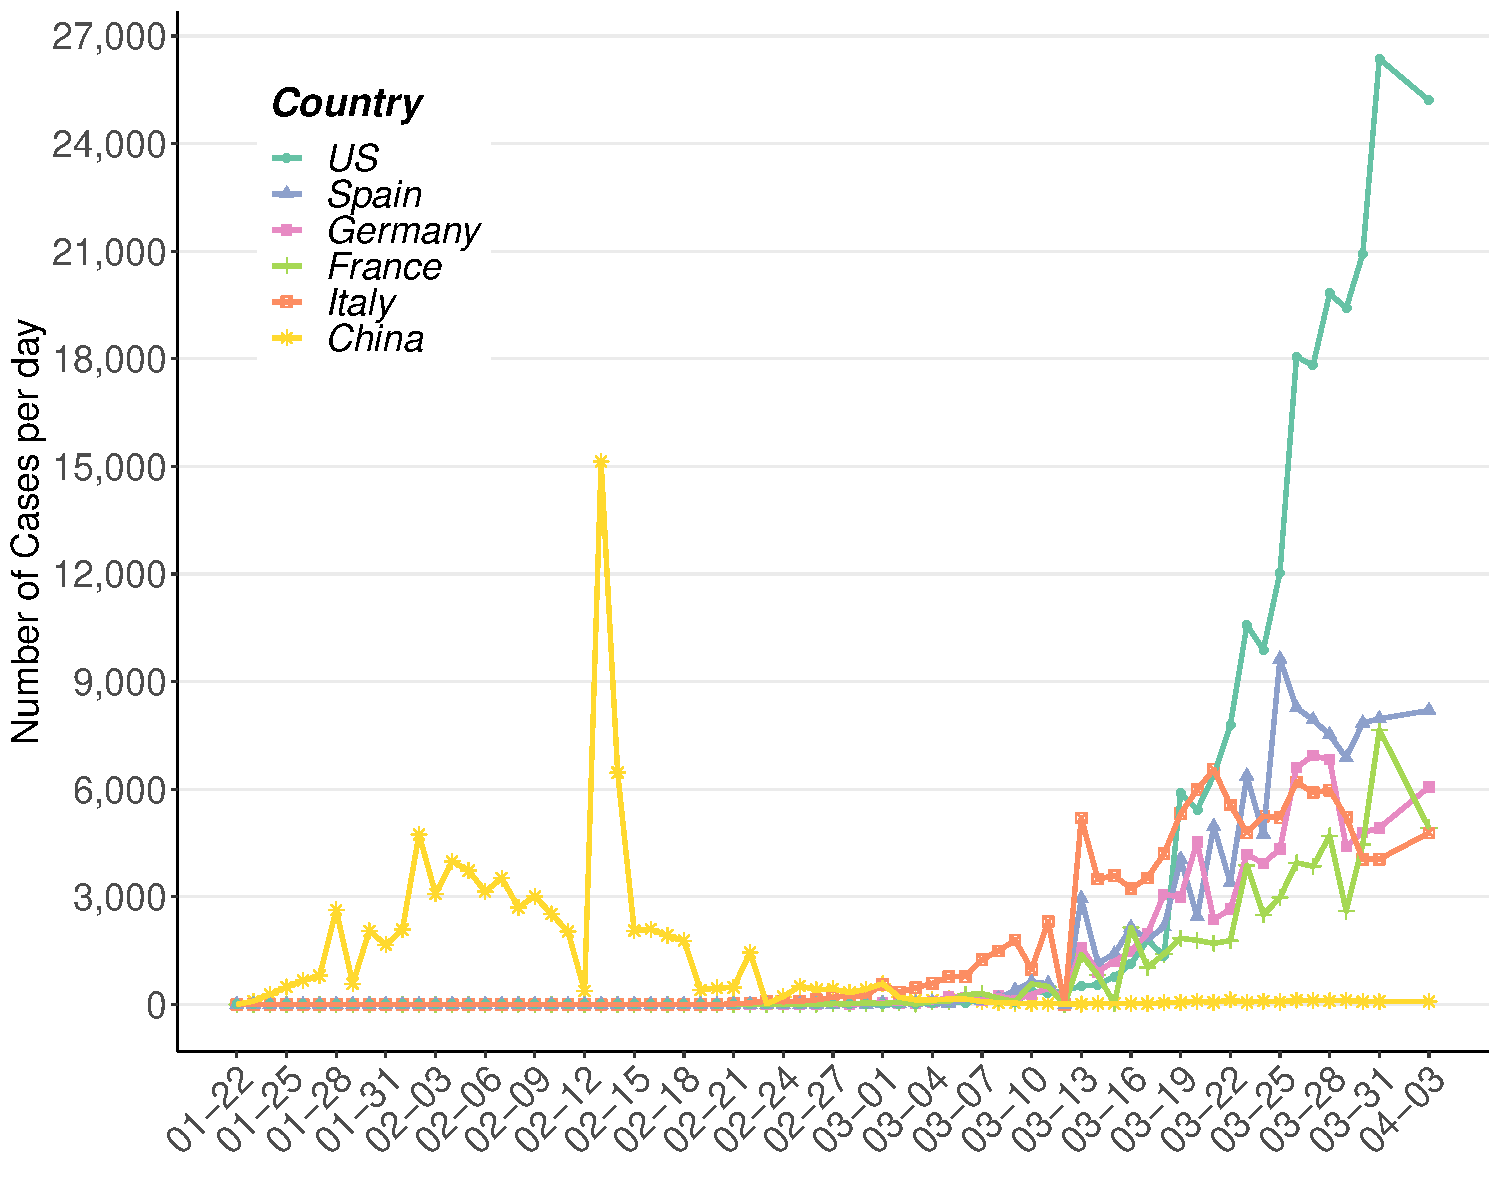
\includegraphics[]{./input/covid2.pdf}
\label{}
\end{minipage}
\quad
\begin{minipage}[b]{0.48\linewidth}
\caption{日新增死亡病例国家趋势图\\(前五位国家) }
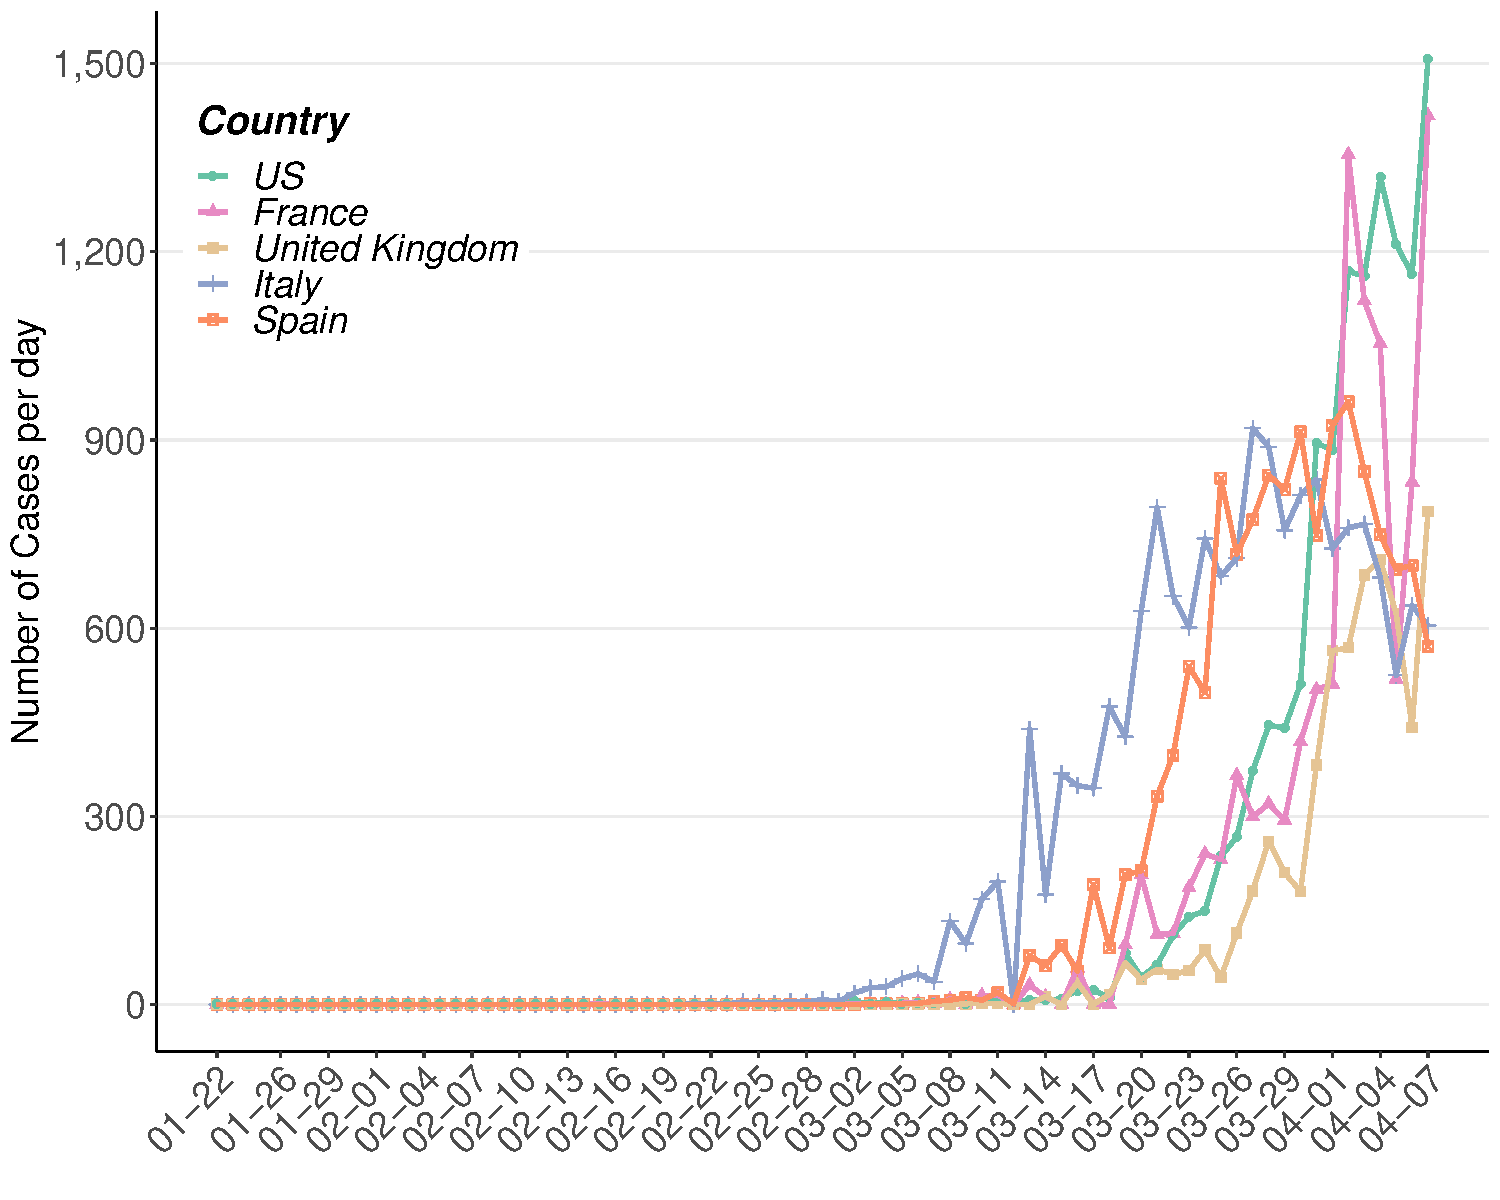
\includegraphics[]{./input/covid3.pdf}
\label{}
\end{minipage}
\end{figure}

\hypertarget{section-3}{%
\section{\texorpdfstring{\textcolor{glaucous}{\Huge 二、美国疫情}}{}}\label{section-3}}

\(\quad\)截至北京时间4月16日早7:00,
美国累计确诊病例数已达到636,350例,共28,326
死亡病例。从州疫情分布图(图4,图5)来看,美国各州疫情严重,前十州都超过一万五千人。中部地区疫情呈快速蔓延趋势。

\(\quad\)纽约州(NY)、新泽西州(NJ)和马萨诸塞州(MA)为美国疫情最严重的三个州。纽约州和新泽西州检测的阳性率仍然居高不下(40\%以上)提示两个州病人数量巨大,医疗资源持续面临巨大压力
(表4)。密歇根州(MI)的阳性率下降至31\%
(表4),提示该州的检测范围扩大,检测能力增强。

\begin{figure}[H] 
\caption{美国本土疫情分布图} %最终文档中希望显示的图片标题
\centering
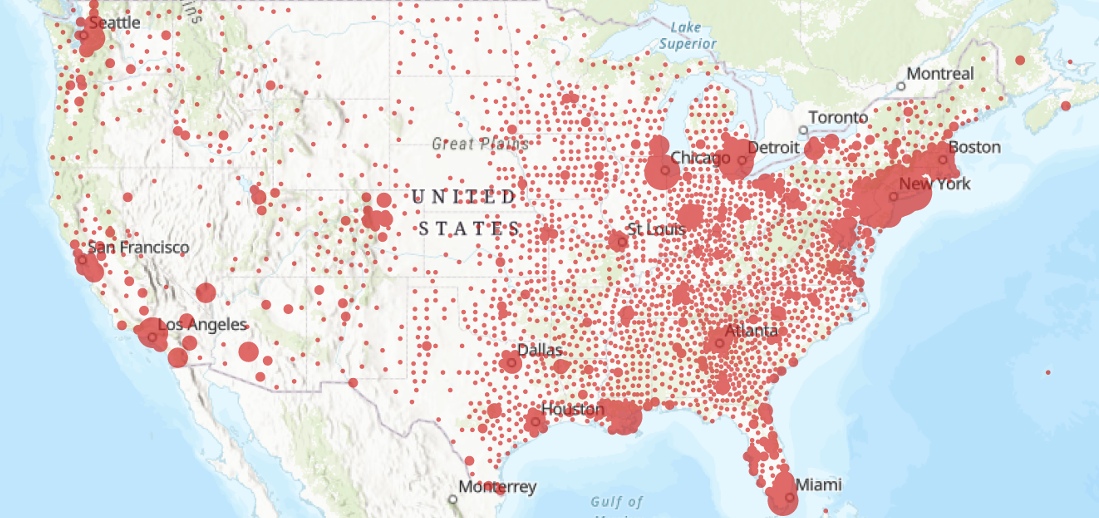
\includegraphics[]{./input/covid4.png} %插入图片,[]中设置图片大小,{}中是图片文件名
\label{} %用于文内引用的标签
\end{figure}

\begin{table}[H]
\vspace{-7mm}
    \caption{美国累计确诊前十位州}
      \vspace{-0.5\baselineskip}
      \centering \begin{table}[H]
\centering\begingroup\fontsize{12}{14}\selectfont

\begin{tabular}{rlrrrrrr}
\toprule
  & 国家/州名 & 累计确诊 & 粗发病率 & 阳性率\% & 累计检测 & 日新增检测 & 检测率\\
\midrule
\rowcolor{gray!6}   & 美国 US & 636,350 & 192 & 20 & 3,242,373 & 161,130 & 980\\
1 & 纽约州 NY & 214,454 & 1,102 & 41 & 526,012 & 26,869 & 2,704\\
\rowcolor{gray!6}  2 & 新泽西州 NJ & 71,030 & 800 & 49 & 144,021 & 4,247 & 1,621\\
3 & 马萨诸塞州 MA & 29,918 & 431 & 23 & 132,023 & 5,472 & 1,900\\
\rowcolor{gray!6}  4 & 密歇根州 MI & 28,059 & 281 & 31 & 89,697 & 3,471 & 898\\
5 & 宾夕法尼亚州 PA & 26,753 & 209 & 19 & 137,584 & 3,953 & 1,075\\
\rowcolor{gray!6}  6 & 加利福尼亚州 CA & 26,686 & 68 & 12 & 216,486 & 14,278 & 548\\
7 & 伊利诺伊州 IL & 24,593 & 194 & 21 & 116,929 & 6,313 & 923\\
\rowcolor{gray!6}  8 & 佛罗里达州 FL & 22,511 & 105 & 11 & 213,509 & 10,329 & 994\\
9 & 路易斯安那州 LA & 21,951 & 472 & 18 & 121,928 & 3,506 & 2,623\\
\rowcolor{gray!6}  10 & 得克萨斯州 TX & 15,907 & 55 & 10 & 151,810 & 5,343 & 524\\
\bottomrule
\end{tabular}
\endgroup{}
\end{table} \begin{tablenotes}
    \fontsize{12}{12}
      \selectfont
    \item 注: 检测率定义:累计检测人数/10万人。计算方式:(累计检测人数/人口)*10万
    \end{tablenotes}
    \end{table}

\begin{figure}[H]
\centering
\begin{minipage}[b]{0.48\linewidth}
\caption{美国日新增确诊前五位州趋势图}
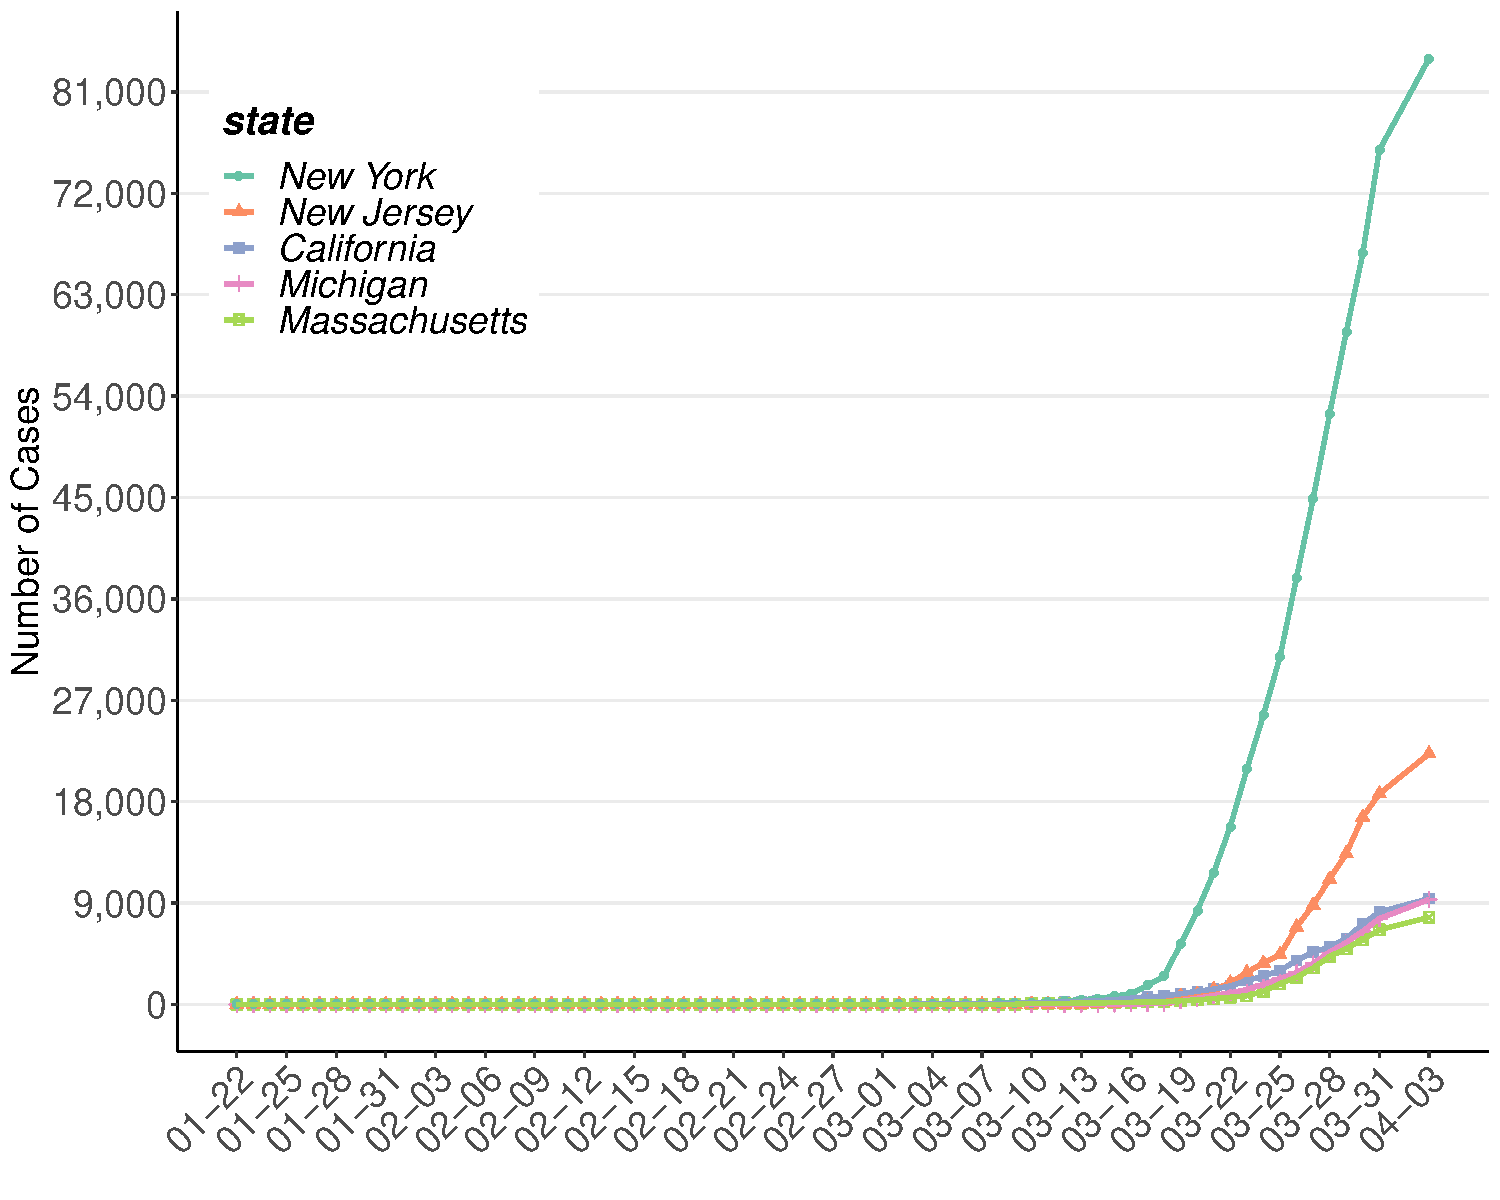
\includegraphics[]{./input/covid5.pdf}
\label{}
\end{minipage}
\quad
\begin{minipage}[b]{0.48\linewidth}
\caption{美国日新增死亡前五位州趋势图}
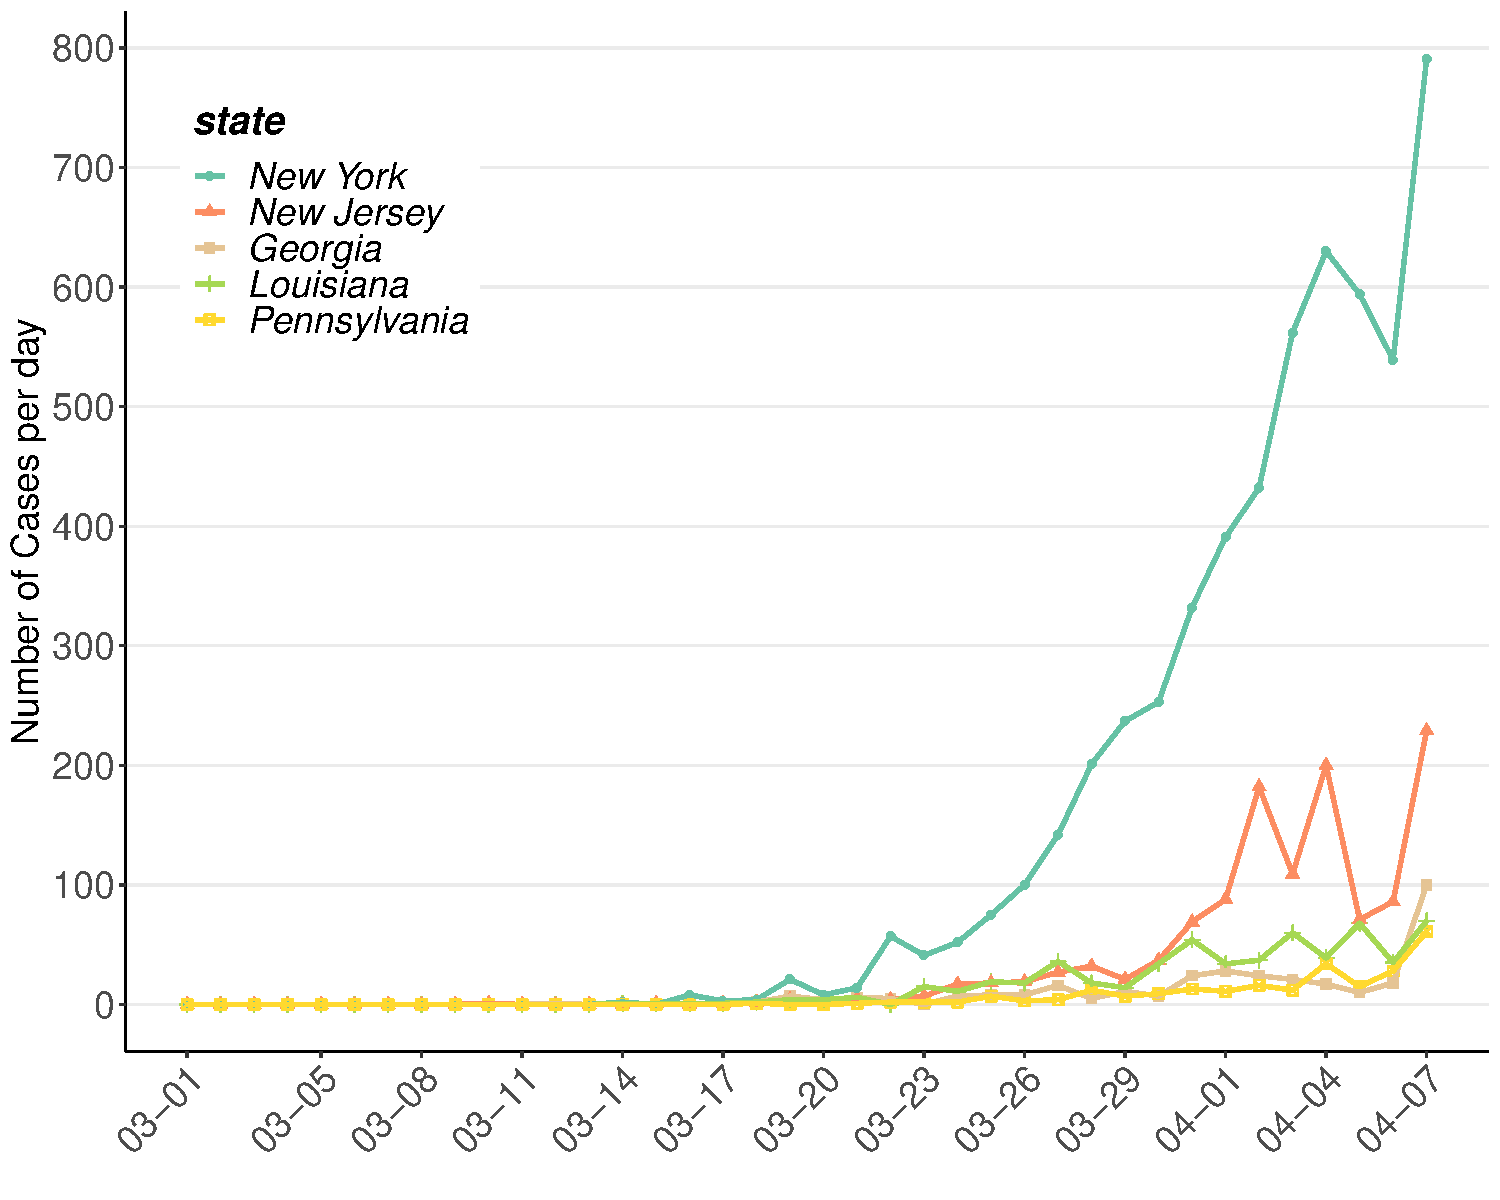
\includegraphics[]{./input/covid6.pdf}
\label{}
\end{minipage}
\end{figure}

\begin{table}[H]
      \centering
    \begin{minipage}{.45\linewidth}
    \caption{美国新增确诊前十位州}
    \vspace{-0.5\baselineskip}
      \centering
    \captionsetup{justification=centering} \begin{table}[H]
\centering\begingroup\fontsize{12}{14}\selectfont

\begin{tabular}{rlrr}
\toprule
  & 国家/州名 & 当日新增 & 构成比\%\\
\midrule
\rowcolor{gray!6}   & 美国 US & 28,680 & 100\\
1 & 纽约州 NY & 11,434 & 40\\
\rowcolor{gray!6}  2 & 新泽西州 NJ & 2,206 & 8\\
3 & 马萨诸塞州 MA & 1,754 & 6\\
\rowcolor{gray!6}  4 & 伊利诺伊州 IL & 1,345 & 5\\
5 & 加利福尼亚州 CA & 1,330 & 5\\
\rowcolor{gray!6}  6 & 宾夕法尼亚州 PA & 1,288 & 4\\
7 & 密歇根州 MI & 1,058 & 4\\
\rowcolor{gray!6}  8 & 得克萨斯州 TX & 901 & 3\\
9 & 佛罗里达州 FL & 883 & 3\\
\rowcolor{gray!6}  10 & 康涅狄格州 CT & 766 & 3\\
\bottomrule
\end{tabular}
\endgroup{}
\end{table} \end{minipage}%
    \begin{minipage}{.45\linewidth}
     \caption{美国累计死亡前十位州}
     \vspace{-0.5\baselineskip}
      \centering
    \captionsetup{justification=centering} \begin{table}[H]
\centering\begingroup\fontsize{12}{14}\selectfont

\begin{tabular}{rlrr}
\toprule
  & 国家/州名 & 累计死亡人数 & 病死率\%\\
\midrule
\rowcolor{gray!6}   & 美国 US & 28,326 & 4.5\\
1 & 纽约州 NY & 11,617 & 5.4\\
\rowcolor{gray!6}  2 & 新泽西州 NJ & 3,156 & 4.4\\
3 & 密歇根州 MI & 1,921 & 6.8\\
\rowcolor{gray!6}  4 & 马萨诸塞州 MA & 1,108 & 3.7\\
5 & 路易斯安那州 LA & 1,103 & 5.0\\
\rowcolor{gray!6}  6 & 伊利诺伊州 IL & 949 & 3.9\\
7 & 康涅狄格州 CT & 868 & 5.9\\
\rowcolor{gray!6}  8 & 加利福尼亚州 CA & 861 & 3.2\\
9 & 宾夕法尼亚州 PA & 779 & 2.9\\
\rowcolor{gray!6}  10 & 佛罗里达州 FL & 596 & 2.6\\
\bottomrule
\end{tabular}
\endgroup{}
\end{table} \end{minipage} 
\end{table}

\(\quad\)纽约州、新泽西州的新增确诊数仍高居前二,其中纽约州较前日增加大约5,000例(表5)。美国共有7个州当日新增病例超过1,000人,
除纽约州外,其余几个州的确诊病例人数近日都在波动 (图5)。

\(\quad\)美国累计死亡病例已突破二万五千例(表6)。纽约州日新增死亡人数近日以来较为稳定,新泽西州,马萨诸塞州和康涅狄格州的日新增死亡人数上升趋势明显(图6)。其他州的日新增死亡人数近日都在波动上升,提示美国疫情仍在恶化。

\hfill\break

%
  \noindent\fcolorbox{lavenderblush}{lavenderblush}{\makebox[\dimexpr\textwidth-2\fboxsep-2\fboxrule][l]{\textbf{~\Huge 案例分析}}}%

\hypertarget{section-4}{%
\section{\texorpdfstring{\textcolor{glaucous}{\Huge 全球卫生体系最薄弱国家之一 — 非洲:塞拉利昂}}{}}\label{section-4}}

\(\quad\)据《金融时报》报道,塞拉利昂750万人口,已有6人被确诊新冠肺炎,可塞拉利昂只有一台呼吸机。这台唯一的呼吸机在当地的一家私人医院,当地17家公立医院均无呼吸机。

\(\quad\)造成塞拉利昂防疫形势严峻的原因有很多。主要原因由如下几点:

\begin{enumerate}
\def\labelenumi{\arabic{enumi}.}
\tightlist
\item
  塞拉利昂是世界上最不发达国家之一,经济发展水平落后,医疗资源匮乏。
  1991-2001,该国经历了长达十年之久的内战。在2014年联合国开发计划署发布的人类发展指数排名中,塞拉利昂排名倒数第五。其首都弗里敦的面积只有整个国
  家的1/200,却承受着这个全国1/5人口的压力,且失业率高达70\%。2017年全国注册医生不到200名。
\item
  塞拉利昂的公共卫生体系发展不全面。塞拉利昂曾经是埃博拉病毒的重灾区,尽管在对抗埃博拉之后政府成立了公共卫生应急处理中心,但是由于国内无法量产抗疫物资,依然需要依靠外国援助来解决相关问题。
\item
  新冠疫情已经在非洲大陆快速扩散。截至4月5日,非洲已有51个国家报告出现新冠确诊病例,累计确诊人数8,736人。而两周前,非洲累计确诊人数仅为1,654
  例。在两周之内,非洲确诊人数就增长了4倍。由于防疫能力和资源有限,塞拉利昂无法同时在控制本土病例的同时兼顾严防输入型病例,使疫情防控雪上加霜\(^1\)。
\end{enumerate}

\(\quad\)我国政府长期以来支持非洲公共卫生事业的发展。早在2016年6月,中非就共同签署了《中华人民共和国商务部和非洲联盟委员会关于开展非洲疾病预防控制中心合作谅解备忘录》。2016年塞拉利昂总统欧内斯特·巴伊·科罗马访问中国时特别到访了中国疾控中心,商议中塞公共卫生技术合作相关事宜\(^2\)。

\(\quad\)目前我国国内疫情局势相对稳定,已大规模复工复产,医用防护服、医用防护口罩/面罩、测温仪、呼吸机产能已基本能满足国内需求,企业也正尽力组织扩大出口\(^3\)。在未来一段时间的抗疫物资援助和贸易上,我国相关产业可更多的将目光放在类似塞拉利昂这样的医疗资源和经济基础更加薄弱的国家。

\Large 参考文献:

\begin{enumerate}
\def\labelenumi{\arabic{enumi}.}
\item
  南财快评之全球疫情观察:从塞拉利昂看非洲防控
  ~\url{https://k.sina.com.cn/article_1651428902_626ece2602000p2bm.html?from=news\&subch=onews}
\item
  塞拉利昂总统访华,为何首站选择疾控中心?~\url{https://mp.weixin.qq.com/s/lf5e9PfSU7LF-3FiNoi72A}
\item
  工信部:中国呼吸机产能无法满足全球疫情防控需求
  ~\url{https://baijiahao.baidu.com/s?id=1663393284129099919\&wfr=spider\&for=pc}
\end{enumerate}

\centering
\fontsize{12}{12}
\selectfont
\begin{tabular}{ll}

主编:马晶  &  副主编:薛成海\,  仁晖  \\
执行责任编辑:王冠  & 责任编辑:乐昊欣\, 闫怡璇 \\
新闻组:张宁\, 张心其  & 数据分析:杜兆慧 \\
案例分析: 史珂玮  &  微信排版:韩佩瑾 \\
\multicolumn{2}{l}{可视化组:张立达\, 孙昊\, 唐星鸿\, 齐维为\, 刘逸洋\,张祺珉\,周梓淇}

\end{tabular}

\end{document}
